\documentclass[../thesis.tex]{subfiles}

\begin{document}

\chapter*{DATA DIRI PENULIS}
\addcontentsline{toc}{chapter}{DATA DIRI PENULIS}

\begin{wrapfigure}[7]{l}{3cm}
\centering
    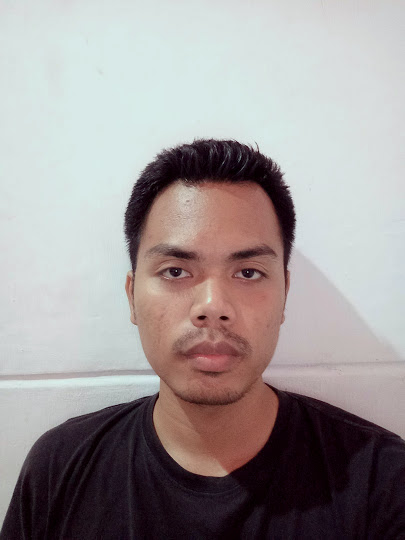
\includegraphics[width=2.8cm,trim=60 40 60 140,clip]{saya.jpg}
\end{wrapfigure}

\noindent Muhammad Uliah Shafar, pria kelahiran Parepare, 26 Juni 1996, sebagai putra sulung dari Parman Farid dan Junaeda. Lulus pendidikan S2 di Magister Arsitektur DAFT Undip, dengan alur konsentrasi Arsitektur Kota. Uliah menjalani pendidikan S2 sejak 2019 sesaat setelah menempuh pendididkan S1nya di UTY Yogyakarta.
Uliah mulai tertarik dengan bidang perkotaan sejak dia menonton film Spiderman sewaktu remaja. Ia melihat scene dimana spiderman berada di bawah jalan raya yang teknisnya disebut sistem pembuangan air kotor kota dan berpikir bahwa tempat tersebut tidak ada di kotanya dan mungkin itu memiliki kegunaan yang besar untuk seisi kota tersebut. Rasa keingintahuan terhadap bagaimana kota terbentuk menjadi latar belakang ia sangat bersemangat dalam menulis dan merancang hal-hal baru berkaitan sebuah kota yang terpelihara dan terorganisir dengan baik.

Saat ini tulisannya sudah ada yang terpublikasikan di jurnal nasional berkaitan dengan ruang publik. Ketekunannya dalam menulis membuatnya ingin merencanakan penulisan artikel-artikel di kemudian hari, bahkan dalam bahasa internasional. Uliah sangat tertarik dengan buku-buku perkotaan terutama dengan judul Making Place. Buku tersebut menurutnya sangat menarik karena dipadukan dengan ilmu sains dan seni praktis dalam menggambarkan realitas sebuah kota.

\vspace{2\baselineskip}
\begin{flushright}
    Hormat saya,\\ Muhammad Uliah Shafar
\end{flushright}


%\onlyinsubfile{\biblio}
\end{document}
